\chapter{Experimentation and results}
\label{Chapter4}

After having explained the necessary theoretical background and presented the proposals
of this work, it is time that we put them into action to see how they perform. First, we are going
to test our proposals on some toy datasets in order to better understand them. After that, we are going
to try the proposed invariants as well as the multiclass extension with ECOC on real data to see how
well they perform when comparing them to the original invariants proposed in \cite{Vapnik2019}.

\section{Experimenting with toy problems}

In this section we will perform a set of simple experiments with some toy datasets. In this case, we have
considered the circles and moons datasets, which can be seen in figure \ref{fig:toy_datasets}. Both of
these problems are available in \texttt{scikit-learn}, which means that we will be able to easily generate
our custom datasets with the available functions. When experimenting with these problems we aim to:

\begin{itemize}
    \item Compare the original invariants with the ones that have been proposed in this work.
    \item Compare the original version of the LUSI algorithm with the ECOC version to see if there is
    any significant difference in a binary setting.
    \item Discover whether some types of invariants are more likely to be selected when considering all types
    of invariants.
\end{itemize}

\begin{figure}[H]
    \centering
    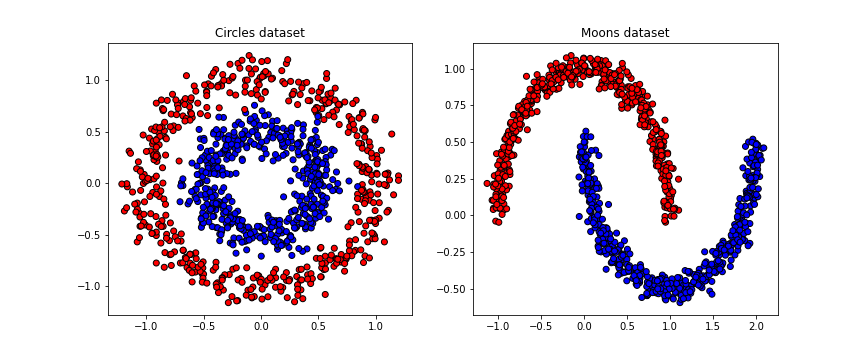
\includegraphics[width=\textwidth]{thesis/Figures/toy_datasets.png}
    \caption{Toy datasets used in the experimentation.}
    \label{fig:toy_datasets}
\end{figure}

\subsection{Experimental settings}

For this experimentation, we have generated one dataset for each problem with a fixed seed. The experimental
parameter settings for each type of problem can be seen in table \ref{tab:toy_problems_experiments}. In an experiment,
we split the data in training and test, keeping 10\% of the data in the training partition and the reamining
90\% in the test partition. We have performed these experiments using Vapnik's invariants and the ones
that we have proposed. As for Vapnik's invariants, we have considered the zeroth and first order invariants, which are

\[
    \psi_0(x) = 1,\quad \psi_1(x) = x_1,\quad \psi_2(x) = x_2
\]

\begin{table}[h]
\centering
\begin{tabular}{llr}
\textbf{Problem} & \textbf{Parameter}  & \textbf{Value} \\ \hline
Circles          & \texttt{n\_samples} & 1000           \\
                 & \texttt{noise}      & 0.1            \\
                 & \texttt{factor}     & 0.5            \\
Moons            & \texttt{n\_samples} & 1000           \\
                 & \texttt{noise}      & 0.05          
\end{tabular}
\caption{Parameter settings of the toy problems.}
\label{tab:toy_problems_experiments}
\end{table}

\subsection{Comparing the different invariant types and versions of LUSI}

In order to compare the two versions of the LUSI algorithm and the different invariants
we have trained a model for each version of LUSI and each invariant type on both problems with a fixed
initial random state. We have visualized the decision boundaries in each case in order to see if there is any
significant difference between them. Additionally, for the LUSI version we have reported the mean number of selected
invariants of each type by repeating the experiment with 10 different initial states. We have limited the
maximum number of invariants of each model to 3 because even though we can generate infinite new random
invariants, we cannot do the same with the original invariants.

Figures \ref{fig:circles_decision_boundary} and \ref{fig:moons_decision_boundary} show the decision
boundaries generated by the original version of the LUSI algorithm whereas figures
\ref{fig:circles_decision_boundary_ecoc} and \ref{fig:moons_decision_boundary_ecoc} display the decision
boundaries of the ECOC version. For the circles problem, we can see that all invariants produce
very similar decision boundaries. In the case of ECOC version, this decision boundary seems to be much
closer to the points of the blue class than in the case of the original algorithm, where the decision boundary
is a bit wider. As for the moons problem, we can observe that the decision boundary is not perfect
in any of the versions of the algorithm since some points fall into the region of the opposite class,
probably caused by to the geometric shape of the both classes. For this problem, the decision boundary seems
to be more accurate using the original algorithm. This is especially true in the case of the random hyperplanes,
where the decision boundary is better adjusted in the case of the original algorithm, whereas it seems that it
has been overfitted when using the ECOC algorithm because we can observe some ``decision islands'' for the blue
class. Overall, it seems that Vapnik's invariants and the random projections produce very similar results
regardless of which version of the algorithm is applied. Hence, if we use any of these two invariants, we
could apply any version of the algorithm and get similar results in a binary classification problem. In the
case of the random hyperplanes, there would be some difference between the results obtained with each version
of the algorithm. As we have seen, depending on the problem, we could get similar results to the ones obtained
using the other two types of invariants.

The idea that Vapnik's invariants and the random projections are similar can be further explored. Figure
\ref{fig:toys_small_num_selected_invariants} show how many invariants have been selected for each problem
on average. We can observe that the mean number of selected invariants is the same for Vapnik's invariants
and the random projections, whereas the number of selected invariants is equal to the maximum number of
invariants in the case of the random hyperplanes. Thus, it seems that the number of invariants that can be
chosen when using Vapnik's invariants and the random projections is limited by the number of dimensions of the
data, as selecting more does not provide any new information. In the case of the random hyperplanes, this is
generally not true as we could keep adding more invariants of this type. This might be caused by the
fact that there is a very large number of hyperplanes that separate the data in two partitions and that
can be used to preserve the proportion of elements that fall on the right side of the hyperplane.
Because of this, many invariants of this type can be selected.

\subsection{Exploring the bias towards certain types of invariants}

Now, we would like to study the scenario in which all types of invariants are considered to see if there is
any kind of bias towards particular types of invariants. For this purpose, we have run a similar experiment to
the previous one using the original version of the LUSI algorithm. We have fit 10 models on both problems
using different random states and setting the maximum number of invariants to 50. In each experiment, the
model could choose among all of the invariant types. For each run, we have computed how many invariants of
each type were selected.

A summary of the results can be seen in figure \ref{fig:toys_mean_num_selected}, where the number of
selected invariants has been averaged for each problem. We can see that the models have not selected any of
Vapnik's invariants. On average, they have chosen 2 random projections per problem, which once again matches
the number of dimensions that these problems have. The models have selected 48 random hyperplanes on average
per problem, which gives more strength to the hypothesis that the number of hyperplane invariants that
can be selected is very large, potentially infinite. Because of this, we can see that when considering
all types of invariants at the same time, it is more likely that the hyperplanes invariant will be selected
because it can contribute with more information.

\section{Experimentation on real data}

After testing our proposals on some toy problems and comparing them to the original work, it is time that we
put them into action on real problems. With this experimentation we want to study the quality of the
new invariants compared to Vapnik's proposals to see if we have achieved our goal of creating general purpose
invariants that can be applied to multiple problems and that allow us to obtain quality results. In this section,
we are going to present the experiments that we have performed as well as the obtained results.

\begin{figure}[H]
    \centering
    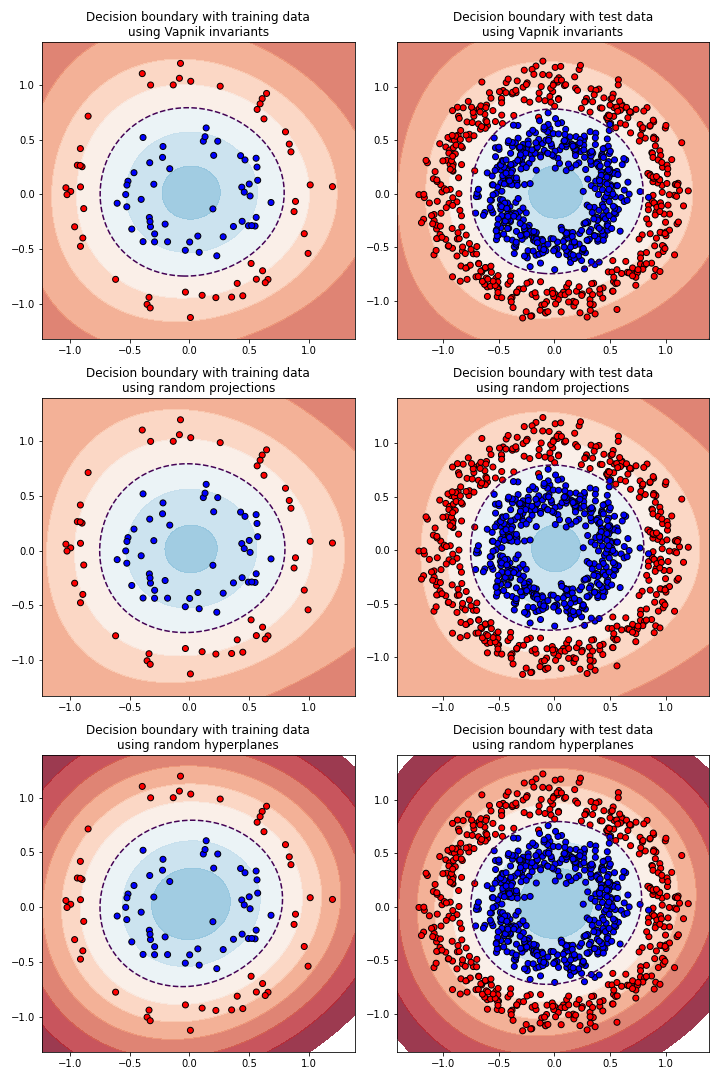
\includegraphics[width=\textwidth]{thesis/Figures/circles_decision_boundaries.png}
    \caption{Decision boundaries in the circles problem using the original LUSI algorithm with each type of
    invariant on the training and test sets.}
    \label{fig:circles_decision_boundary}
\end{figure}

\begin{figure}[H]
    \centering
    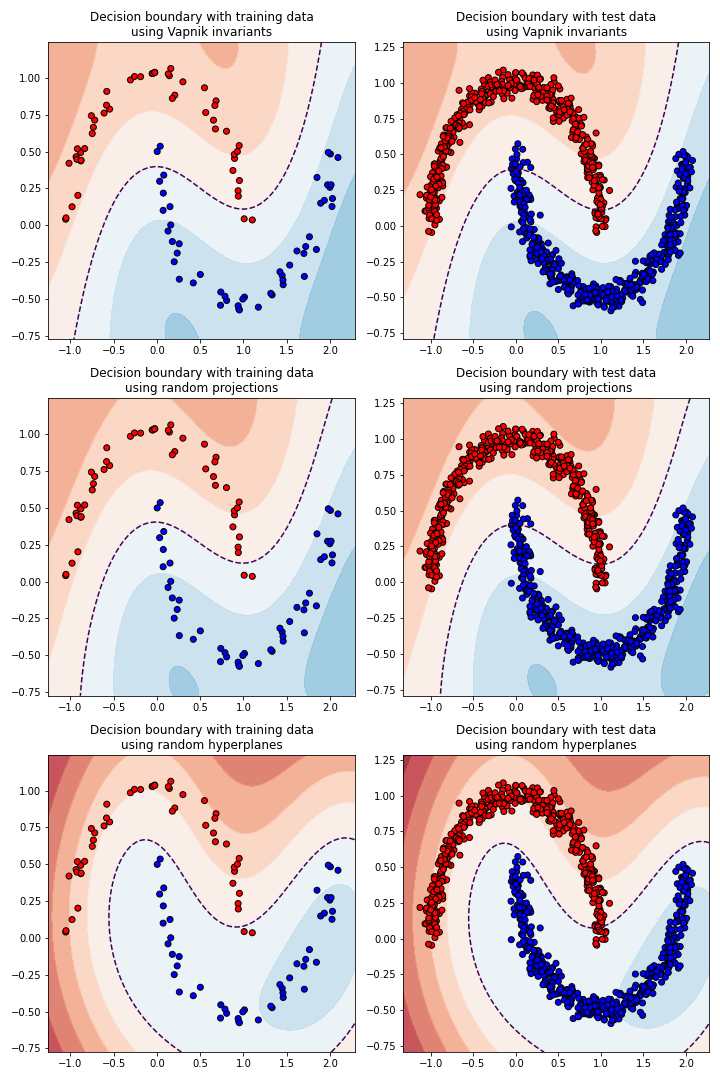
\includegraphics[width=\textwidth]{thesis/Figures/moons_decision_boundaries.png}
    \caption{Decision boundaries in the moons problem using the original LUSI algorithm with each type of
    invariant on the training and test sets.}
    \label{fig:moons_decision_boundary}
\end{figure}

\begin{figure}[H]
    \centering
    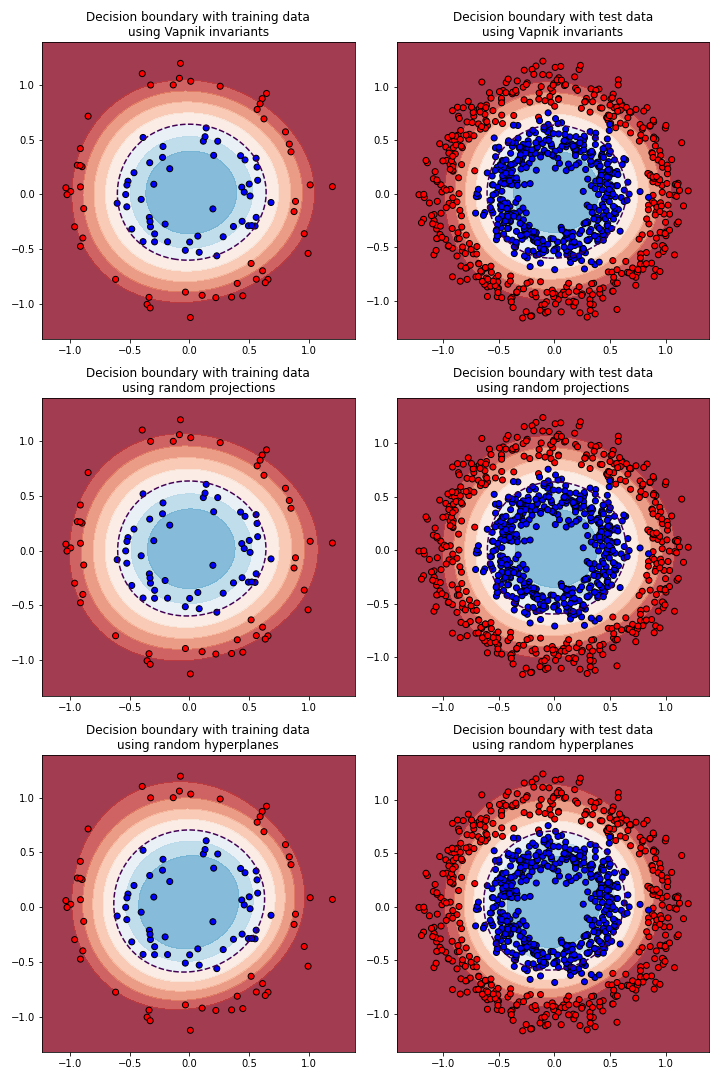
\includegraphics[width=\textwidth]{thesis/Figures/circles_decision_boundaries_ecoc.png}
    \caption{Decision boundaries in the circles problem using the ECOC version of the LUSI algorithm with each type
    of invariant on the training and test sets.}
    \label{fig:circles_decision_boundary_ecoc}
\end{figure}

\begin{figure}[H]
    \centering
    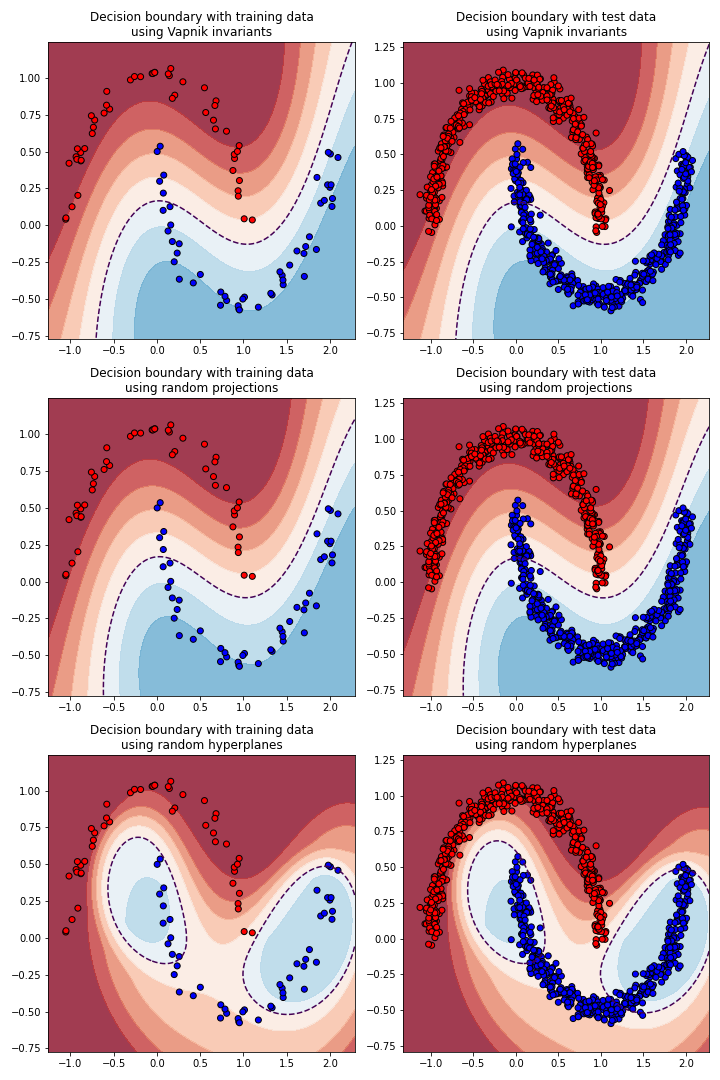
\includegraphics[width=\textwidth]{thesis/Figures/moons_decision_boundaries_ecoc.png}
    \caption{Decision boundaries in the moons problem using the ECOC version of the LUSI algorithm with each type
    of invariant on the training and test sets.}
    \label{fig:moons_decision_boundary_ecoc}
\end{figure}

\begin{figure}[H]
    \centering
    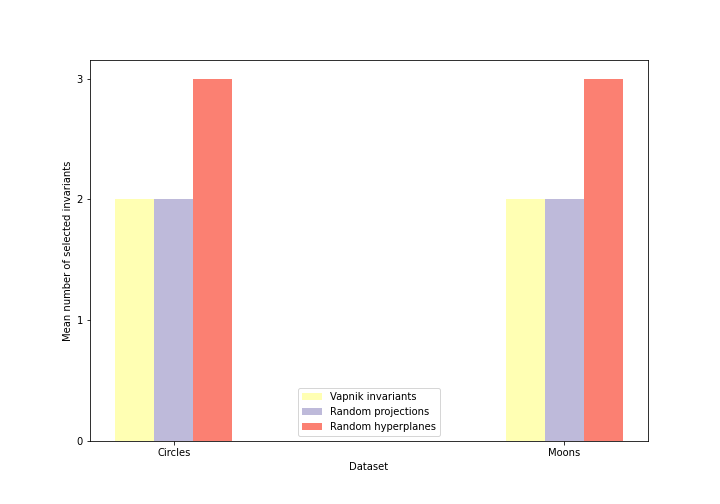
\includegraphics[width=0.8\textwidth]{thesis/Figures/num_selected_invariants.png}
    \caption{Mean number of selected invariants per problem. The maximum number of invariants was set to 3.}
    \label{fig:toys_small_num_selected_invariants}
\end{figure}

\begin{figure}[H]
    \centering
    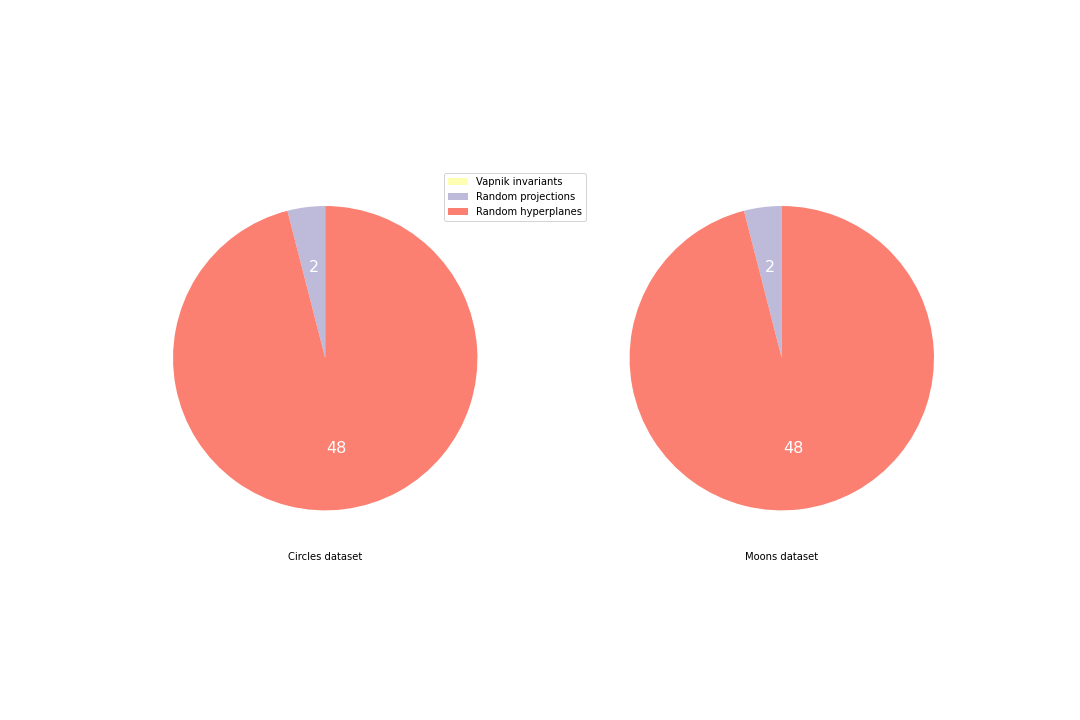
\includegraphics[width=\textwidth]{thesis/Figures/mean_num_selected.png}
    \caption{Mean number of selected invariants when the maximum number of invariants is 50 and the three types of
    invariants are considered simultaneously.}
    \label{fig:toys_mean_num_selected}
\end{figure}


\subsection{Experimental settings}

First and foremost, we need to discuss what datasets we are going to use in the experimentation, what
will be compared and how the experiments will be performed.

As for the data, we are going to use five datasets from the UCI repository (\cite{UCIRepository}). Originally, we
planed on using more datasets, but due to strong time restrictions and the fact that each experiment took from a couple
of hours up to a couple of days it did not seem worthwhile increasing the number of datasets. The selected datasets
along with some basic information about them can be found in table \ref{tab:problems_description}. As we can see, all
of them are multiclass classification problems, which means that we must use the ECOC-based extension that we have
proposed in this work. We applied some preprocessing to the datasets before using them in our experiments, like
transforming the categorical values using hashing and transforming the classes to numerical values so that we
could more easily create the encoding matrices and apply the posterior decoding step.

\begin{table}[H]
\centering
\begin{tabular}{lrrr}
\textbf{Problem} & \textbf{Num. examples} & \textbf{Attributes} & \textbf{Classes} \\ \hline
Balance Scale    & 625                    & 4                   & 3                \\
Ecoli            & 336                    & 8                   & 8                \\
Glass            & 214                    & 9                   & 7(6)\tablefootnote{According to the dataset's documentation, there are 7 classes. However, there is one that does not have any elements. Therefore, the actual number of classes for this problem is 6.}                \\
Iris             & 150                    & 4                   & 3                \\
Yeast            & 1484                   & 8                   & 10              
\end{tabular}
\caption{Information of the datasets used in the experimentation.}
\label{tab:problems_description}
\end{table}

In these experiments, we will be comparing four different versions of LUSI using different types of invariants:
\begin{enumerate*}[label=(\roman*)]
    \item a baseline version with no invariants,
    \item Vapnik's invariants (zeroth and first order invariants),
    \item random projections and
    \item random hyperplanes.
\end{enumerate*}

In order to compare the different models, we have designed an experimentation methodology that we will briefly
describe. We are going to create three different stratified partitions of each dataset using different seeds.
In these partitions we are going to keep 80\% of the data for training and the remaining 20\% will be used to
test the models. For each training partition, we are going to create three different stratified subsamples of it,
keeping 100\%, 50\% and 10\% of the data. Using each one of these subsamples, we are going to perform three grid
searches using 3-fold cross validation over different combinations of hyperparameters for each one of the models,
finding the best possible combination of hyperparameters in each case. Finally, we are going to evaluate these
models using the test set from the corresponding partition and obtain a accuracy for that particular scenario.
We are using the same test partition to evaluate the different models so that we can have a common ground that allows
us to fairly compare the different types of invariants. A general overview of this experimentation methodology
can be seen in figure \ref{fig:experimentation_setup}, where an example is shown using the random projections
invariant.

Finally, we need to clarify which hyperparameters we are going to be fine-tuning. For this experimentation and due
to the previously mentioned time restriction as well as the hefty amount of hyperparameter combinations for each
model, we have restricted ourselves to performing the grid search on the following hyperparameters:

\begin{itemize}
    \item The maximum number of invariants that can be selected.
    \item The value of $\delta$ used in the invariants selection.
    \item The value of $\gamma$ used when computing the kernel.
    \item The value of \texttt{C}, which is a regularization parameter that controls how much perturbation
    is applied to the product of the $V$ and $K$ matrices before computing the inverse so that it is not a
    singular matrix.
\end{itemize}

\begin{figure}[h]
    \centering
    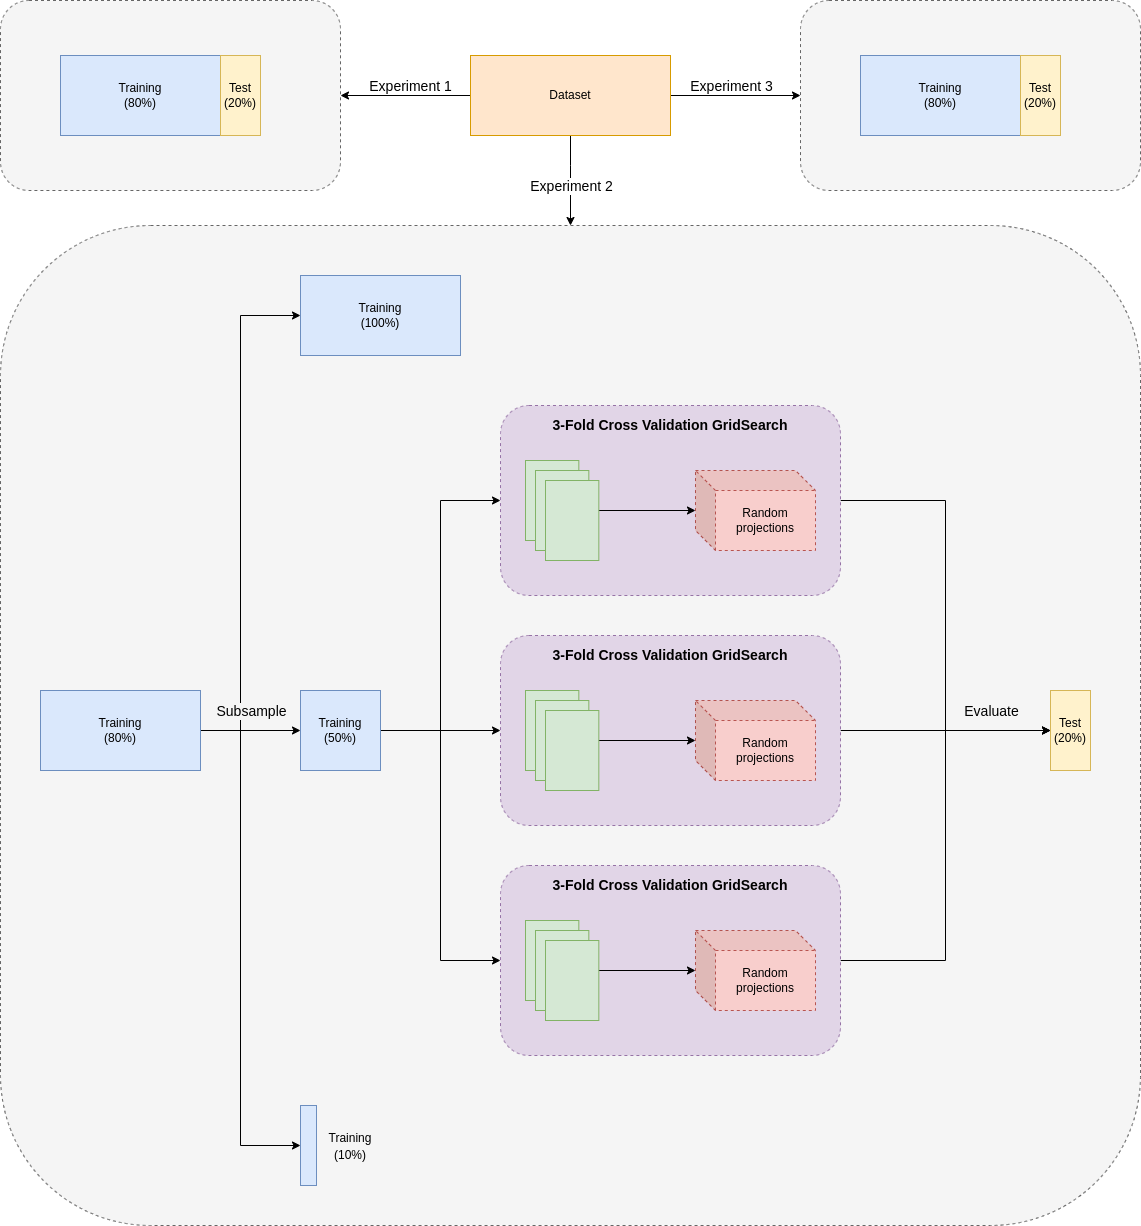
\includegraphics[width=\textwidth]{thesis/Figures/experimentation_scheme.drawio.png}
    \caption{Overview of the experimentation methodology. In this example, the grid search is only applied to
    the random projections model for a subsample of 50\% of the training partition, although in a real scenario
    it would be applied to each training subsample and to each type of model. Note that all models are evaluated using
    the same test partition.}
    \label{fig:experimentation_setup}
\end{figure}

\subsection{Results}

Let us now analyze the results that we have obtained from the experimentation. Tables
\ref{tab:results_accuracies_errors_100} and \ref{tab:results_accuracies_errors_10}
contain the mean accuracies and standard deviations for each dataset considering the different invariant types
and training subsample sizes. We have only reported the mean accuracies achieved when using a subsample
of 100\% and 10\% of the training partitions, as they represent two extremes of the learning problem: one in which
there is a lot of available training data, and one where this data is scarce.

We can observe that the baseline model with no invariants almost completely outperforms the rest of the
models which use some kind of invariants on both training sizes. Also, it is the one that has the
least variation in the results. In second place we find the original invariants proposed by Vapnik, which
offer good results overall, although a model that uses no invariants is capable of achieving better results.
The random projections follow quite closely Vapnik's invariants, offering average results that are a bit worse
than the original invariants. However, they are capable of achieving better results than Vapnik's invariants in
the Balance Scale dataset using a big training size and in the Glass dataset when considering a small training
dataset. The large deviation in the Iris dataset in the small problem is really curious, probably caused by a
bad random seed. Finally, the random hyperplanes come in last place, offering the worst results in almost all
problems irregardless of the training size.

One possible explanation for the poor results obtained by the random invariants may be that the random
seeds that we have chosen are quite bad. Because these invariants heavily rely on stochastic processes,
a bad initialization can greatly worsen the results. Thus, we can try to repeat these
experiments with more carefully selected random seeds or by increasing the pool of initial seeds, which
would mean that we would have to run more experiments, which as we have already mentioned, takes a very long
time and computational resources.

This randomness also affects the variation of the results. As we can clearly see, the models that use the
random invariants have larger standard deviations. Because the model that uses no invariants has no
need to select invariants and the one that uses Vapnik's proposed invariants does not have to generate new
invariants, the training process becomes more deterministic, which reduces the overall variability of the results.

Another result that must be highlighted is the poor performance of the random hyperplanes. A possible
explanation of this might be that this invariant is a modification of the zeroth order invariant in
which the proportion of elements is only kept in a region of the original space. Although the idea seemed
interesting in the first place as we have potentially infinite hyperplanes that can separate the data in order
to keep different proportions of it, in practice it seems that preserving this kind of statistical information
might not be that useful as the models may be prone to overfitting, as we saw in the experimentation with the toy
problems.


\begin{table}[h]
\centering
\resizebox{\textwidth}{!}{%
\begin{tabular}{lcccc}
\textbf{Dataset} & \textbf{Baseline model} & \textbf{Vapnik invariants} & \textbf{Random projections} & \textbf{Random hyperplanes} \\ \hline
Balance Scale & $91.47 \pm 0.38\%$ & $91.47 \pm 0.38\%$ & $91.73 \pm 0.38\%$ & $90.13 \pm 1.51\%$  \\
Ecoli         & $85.29 \pm 2.08\%$ & $85.29 \pm 1.20\%$ & $84.15 \pm 2.05\%$ & $75.98 \pm 6.28\%$  \\
Glass         & $72.87 \pm 7.91\%$ & $72.87 \pm 7.91\%$ & $72.09 \pm 7.44\%$ & $71.06 \pm 7.60\%$  \\
Iris          & $96.67 \pm 0.00\%$ & $95.56 \pm 1.57\%$ & $95.19 \pm 1.66\%$ & $88.52 \pm 11.56\%$ \\
Yeast         & $53.76 \pm 1.04\%$ & $53.87 \pm 1.20\%$ & $52.53 \pm 5.44\%$ & $50.39 \pm 5.33\%$ 
\end{tabular}%
}
\caption{Mean accuracy and standard deviation for each type of invariant in each problem considering the results for subsamples of 100\% of the training data. The results are expressed as percentages.}
\label{tab:results_accuracies_errors_100}
\end{table}

\begin{table}[h]
\centering
\resizebox{\textwidth}{!}{%
\begin{tabular}{lcccc}
\textbf{Dataset} & \textbf{Baseline model} & \textbf{Vapnik invariants} & \textbf{Random projections} & \textbf{Random hyperplanes} \\ \hline
Balance Scale & $88.80 \pm 1.73\%$ & $87.73 \pm 2.10\%$ & $83.73 \pm 7.17\%$  & $76.00 \pm 12.77\%$ \\
Ecoli         & $71.57 \pm 1.39\%$ & $72.55 \pm 4.22\%$ & $67.32 \pm 4.03\%$  & $63.89 \pm 9.61\%$  \\
Glass         & $56.59 \pm 4.78\%$ & $45.74 \pm 6.67\%$ & $52.45 \pm 7.03\%$  & $45.48 \pm 9.50\%$  \\
Iris          & $93.33 \pm 2.72\%$ & $90.00 \pm 4.71\%$ & $77.78 \pm 22.93\%$ & $84.81 \pm 9.04\%$  \\
Yeast         & $47.92 \pm 2.08\%$ & $47.92 \pm 2.14\%$ & $45.68 \pm 4.60\%$  & $37.82 \pm 7.92\%$ 
\end{tabular}%
}
\caption{Mean accuracy and standard deviation for each type of invariant in each problem considering the results for subsamples of 10\% of the training data. The results are expressed as percentages.}
\label{tab:results_accuracies_errors_10}
\end{table}

We can delve into the previous results by comparing how many times each model obtains a better, worse
or the same accuracy as the rest of the models for the same experiment. This information has been
condensed in figures \ref{fig:invariants_performance_1} and \ref{fig:invariants_performance_2}, where we
can see the performance of the different models across all experiments.

As we can observe, the model with no invariants is capable of achieving more times greater accuracies than
the rest of the models irregardless of the training size. When compared to the model that uses Vapnik's invariants,
we can see that they achieve the same accuracy in a lot of experiments (approximately 50\% of the times). This
model offers worse results in only a couple of experiments, which are less than 20\% of the times. Something similar
happens when we compare it to the random projections, although the results are a bit more favorable for the model
with no invariants in this case. When comparing it to the random hyperplanes, we can see that the latter one
is totally outmatched.

If we compare now Vapnik's invariants to the random projections, we can see that they achieve very similar
results overall, although they are more favorable in the case of Vapnik's invariants. When comparing
these invariants with small training sizes, we can see that the difference between them is less significant.
Hence, as we saw in the previous experimentation and in this one, we can state that these types of invariants are
very similar. Probably, this is due to the fact that most of Vapnik's invariants are first order invariants,
and the random projections are a variation of this type of invariant. With them, we can preserve the centroid of
each class, which is an interesting information that should be kept when learning the bets approximation of the
target function.

Finally, to no one's surprise, the random hyperplanes are the ones that perform the worst when compared to the
rest of the models, as it is the invariant type that gets beaten the most frequently. This might be because the
information provided by this variation of the zeroth order invariant is not as relevant as the one provided by
the original zeroth order invariant or higher order invariants. Hence, its usefulness seems questionable even
when a model that uses no invariants is capable of outperforming a model that uses this kind
of invariant by far.

\begin{figure}[ht]
    \centering
    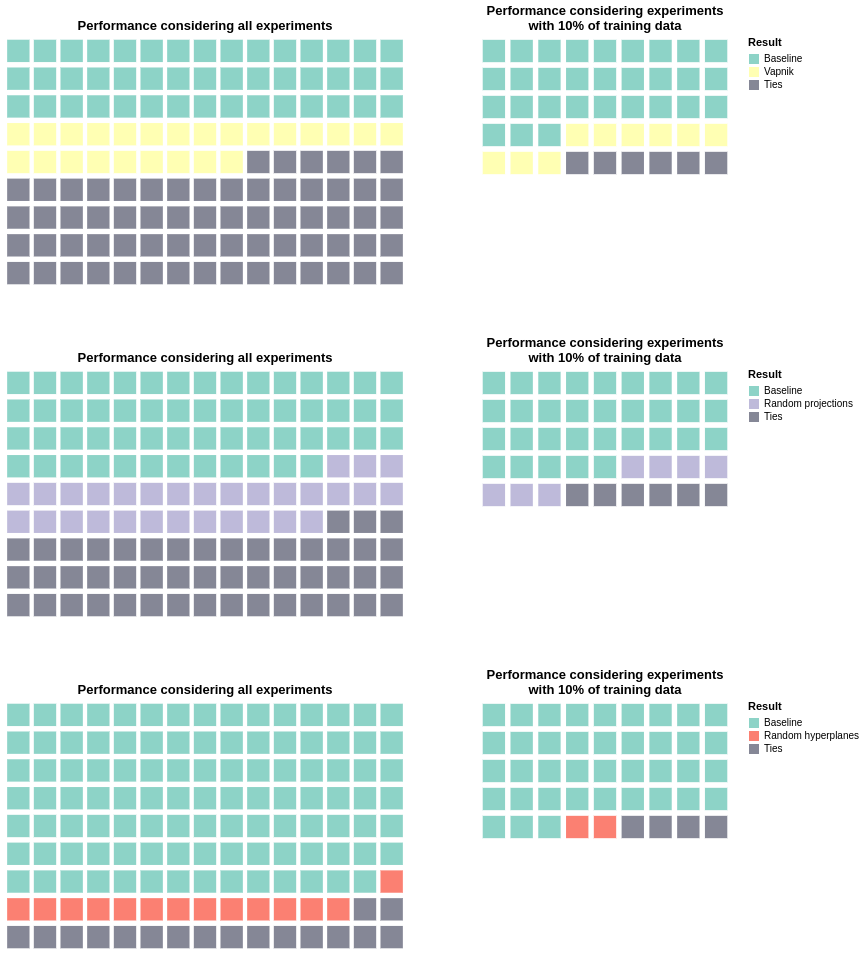
\includegraphics[width=\textwidth]{thesis/Figures/invariants_performance_1.png}
    \caption{Number of times that the baseline model achieves a better, worse or the same
    accuracy when compared to the rest of the models in the same experiment,
    aggregated across all datasets. Left column shows the results obtained when the training size is disregarded.
    The right one shows the results only when considering the experiments where 10\% of the training partition
    is used.}
    \label{fig:invariants_performance_1}
\end{figure}

\begin{figure}[ht]
    \centering
    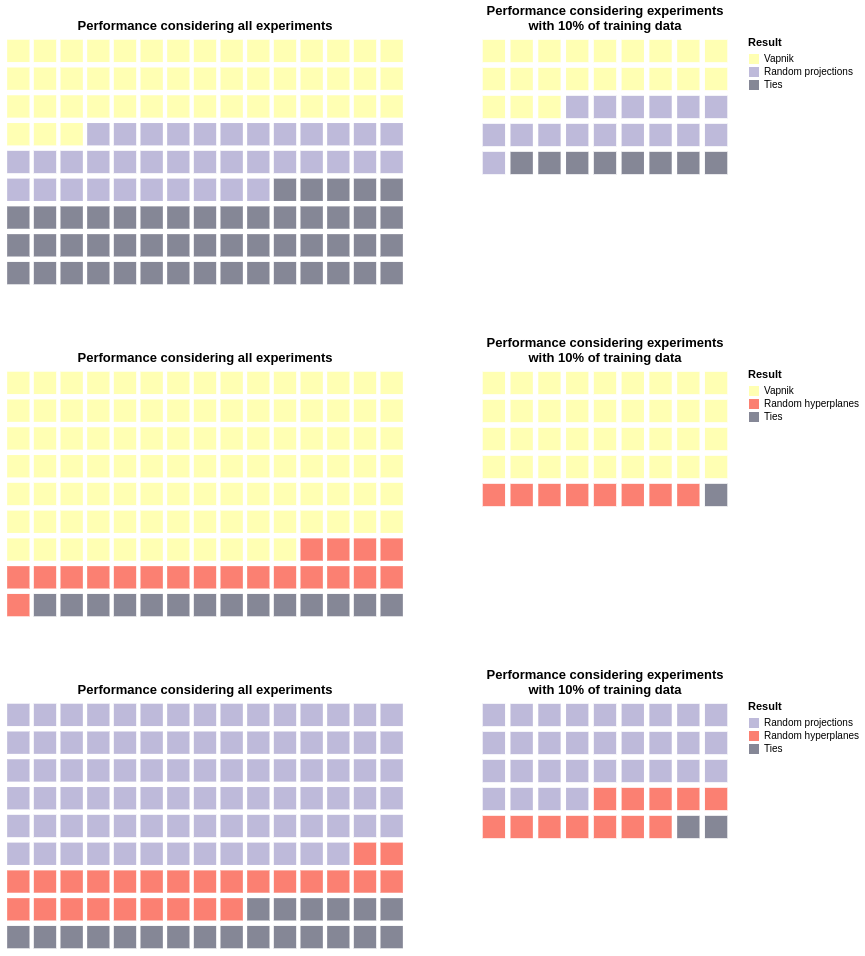
\includegraphics[width=\textwidth]{thesis/Figures/invariants_performance_2.png}
    \caption{Number of times that the models using Vapnik's invariants, random projections and
    random hyperplanes achieve a better, worse or the same accuracy when compared one to another
    in the same experiment, aggregated across all datasets. Left column shows the results obtained when
    the training size is disregarded. The right one shows the results only when considering the experiments
    where 10\% of the training partition is used.}
    \label{fig:invariants_performance_2}
\end{figure}